\documentclass[a4paper,10pt]{article}
\usepackage{tikz}
\usepackage{verbatim}
\usepackage[margin=15mm]{geometry}
\usetikzlibrary{shapes,arrows,fit,calc,positioning}


\begin{document}

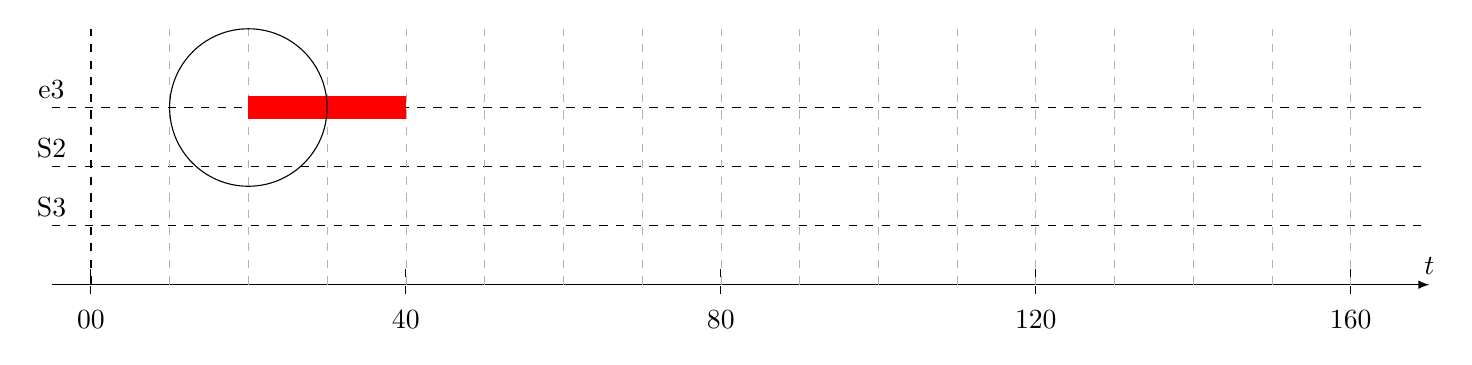
\begin{tikzpicture}[xscale=1,transform shape]

% Idõtengely rajzolása
\draw [-latex](-0.5,0) coordinate(dd)-- (0,0) coordinate (O1) -- (17,0)coordinate(ff) node[above]{$t$};

% Kezdő függőleges szaggatott vonal
\draw [dashed,thick] (O1) -- (0,0.75) coordinate(S3) -- (0,1.5) coordinate(S2) -- (0,2.25) coordinate(e3) -- ++(0,1)coordinate(ff2);

% Taszk feliratok a hozzájuk tartozó vonallal
\foreach \nn in{S3,S2,e3}{
\draw [dashed,very thin] (dd|-\nn) node[above]{\nn}-- (\nn-|ff);
}

% Függőleges osztások
\foreach \xx in{1,2,...,16}{
\draw[dashed,black!30!white,very thin] (\xx,0) -- (\xx,0|- ff2);
}

% Időtengely feliratok
\foreach \xx in{0,4,8,...,16}{
\draw[dashed] (\xx,0.2) -- (\xx,-0.2) node[below]{\xx 0};
}

% Taszk téglalap
%\begin{scope}[shift={(e3)}]
%\node[ above right=0.25cm and 0cm of e3,right,draw, minimum width=4cm,minimum height=0.5cm,fill=white](n3a) {$3=f(e_3)$};
%\draw[-latex,thick] (n3a.north west) -- ++(0,0.5)node[right]{$a^{e3}_{3=f(e3)}$};
%\end{scope}

% Taszk vonal
\begin{scope}[shift={(e3)}]
\draw[red, line width=3mm] (2,0) -- (4,0);
\draw (2,0) circle (1cm);
\end{scope}

% Taszk téglalap
%\begin{scope}[shift={(S2)}]
%\coordinate(O2) at (2,0);
%\node[ above right=0.4cm and 0cm of O2,right,draw, minimum width=4cm,minimum height=0.8cm,fill=white](n4a) {$4=f(s_2)$};
%\draw[-latex,thick,green] (n4a.north west) -- ++(0,0.5)node[right,fill=white]{$a^{S2}_{f(S2)}$};
%\draw[-latex,thick,blue] ([xshift=2.7cm]n4a.north west) coordinate(bb1)-- ++(0,0.5)node[right,fill=white]{$a^{S2}_{3=f(e3)}$};
%\draw[dashed,red] (n3a.south east) -- (bb1);
%\node[right=0cm of n4a,right,draw, minimum width=4cm,minimum height=0.8cm,fill=white](n3b) {$3=p(e_3)$};
%\end{scope}

% Taszk téglalap
%\begin{scope}[shift={(S3)}]
%\coordinate(O3) at (0.5,0);
%\node[ above right=0.4cm and 0cm of O3,right,draw, minimum width=4cm,minimum height=0.8cm,fill=white](n1) {$1=f(s_2)$};
%\node[right=0cm of n1,right,draw, minimum width=4cm,minimum height=0.8cm,fill=white](n5) {$5$};
%\node[right=0cm of n5,right,draw, minimum width=4cm,minimum height=0.8cm,fill=white](n4b) {$4=p(S2)$};
%\node[right=0cm of n4b,right,draw, minimum width=4cm,minimum height=0.8cm,fill=white](n3c) {$3$};
%\end{scope}

\end{tikzpicture}

\end{document}

% source: http://tex.stackexchange.com/questions/57533/how-to-draw-a-diagram-for-packets-scheduling-in-networks-or-task-scheduling